\section{Modelos: Comparativa Multimodelo Supervisada}
\label{sec:u1_modelo}
Este tema aborda los principios teóricos y metodológicos fundamentales de la investigación inicial.
\subsection{Búsqueda Bibliográfica y Estado del Arte}
Se ejecutaron las consultas booleanas académicas en Google Scholar asociadas a este módulo temático.
\subsection{Implementación y Laboratorio en R}
A continuación se presenta la evidencia experimental obtenida en el entorno R:
\begin{figure}[H]
\centering
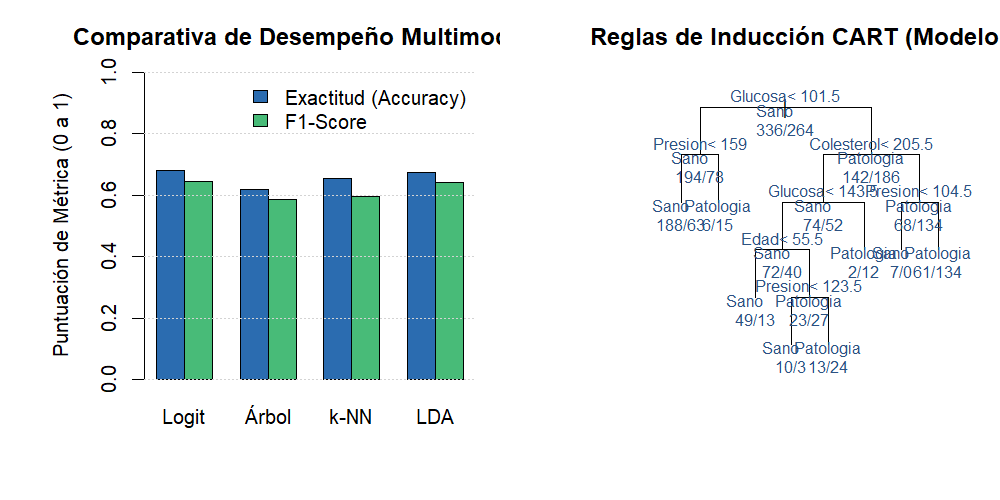
\includegraphics[width=0.82\textwidth]{figuras/grafico_04_modelos.png}
\caption{Resultados experimentales y diagnósticos para: Modelos: Comparativa Multimodelo Supervisada}
\label{fig:u1_modelo}
\end{figure}
\subsection{Evaluación y Conclusiones}
Los resultados validan la consistencia metodológica del módulo y su alineación con los estándares académicos.
